\documentclass[journal]{vgtc}                % final (journal style)

\ifpdf%                                % if we use pdflatex
  \pdfoutput=1\relax                   % create PDFs from pdfLaTeX
  \pdfcompresslevel=9                  % PDF Compression
  \pdfoptionpdfminorversion=7          % create PDF 1.7
  \ExecuteOptions{pdftex}
  \usepackage{graphicx}                % allow us to embed graphics files
  \DeclareGraphicsExtensions{.pdf,.png,.jpg,.jpeg} % for pdflatex we expect .pdf, .png, or .jpg files
\else%                                 % else we use pure latex
  \ExecuteOptions{dvips}
  \usepackage{graphicx}                % allow us to embed graphics files
  \DeclareGraphicsExtensions{.eps}     % for pure latex we expect eps files
\fi%

%% it is recomended to use ``\autoref{sec:bla}'' instead of ``Fig.~\ref{sec:bla}''
\graphicspath{{figures/}{pictures/}{images/}{./}} % where to search for the images

\usepackage{microtype}                 % use micro-typography (slightly more compact, better to read)
\PassOptionsToPackage{warn}{textcomp}  % to address font issues with \textrightarrow
\usepackage{textcomp}                  % use better special symbols
\usepackage{mathptmx}                  % use matching math font
\usepackage{times}                     % we use Times as the main font
\renewcommand*\ttdefault{txtt}         % a nicer typewriter font
\usepackage{cite}                      % needed to automatically sort the references
\usepackage{tabu}                      % only used for the table example
\usepackage{booktabs}                  % only used for the table example

\onlineid{0}

\vgtccategory{Research}

\vgtcpapertype{system}

%% Paper title.
\title{DSOC: Decision Support for Organizational Change}

\author{Rob Barwell and Eric Sper}
\authorfooter{
%% insert punctuation at end of each item
\item
 Rob Barwell and Eric Spero are with Carleton University. E-mail: robert.barwell/eric.spero@carleton.ca.
}

%other entries to be set up for journal
\shortauthortitle{Biv \MakeLowercase{\textit{et al.}}: Global Illumination for Fun and Profit}
%\shortauthortitle{Firstauthor \MakeLowercase{\textit{et al.}}: Paper Title}

\abstract{
  Our abstract goes here.
} 
\keywords{Organizational change, decision-making, information visualization}

%% ACM Computing Classification System (CCS). 
%% See <http://www.acm.org/class/1998/> for details.
%% The ``\CCScat'' command takes four arguments.

\CCScatlist{ % not used in journal version
 \CCScat{K.6.1}{Management of Computing and Information Systems}%
{Project and People Management}{Life Cycle};
 \CCScat{K.7.m}{The Computing Profession}{Miscellaneous}{Ethics}
}

%% Uncomment below to include a teaser figure.
\teaser{
  \centering
  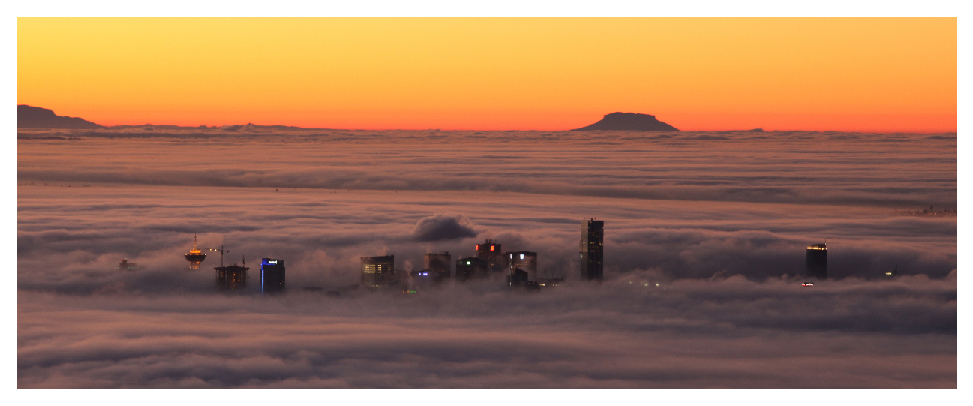
\includegraphics[width=\linewidth]{CypressView}
  \caption{In the Clouds: Vancouver from Cypress Mountain. Note that the teaser may not be wider than the abstract block.}
	\label{fig:teaser}
}

%% Uncomment below to disable the manuscript note
\renewcommand{\manuscriptnotetxt}{}

%% Copyright space is enabled by default as required by guidelines.
%% It is disabled by the 'review' option or via the following command:
%\nocopyrightspace

\vgtcinsertpkg

%% Start document!

\begin{document}

\firstsection{Introduction}

\maketitle
The idea of organizational change has started to shift over the past decade with the introduction of the gig economy and other non-traditional employment models.  Historically a person would obtain a job after high school and university and stay with the same company until retirement.  This has fundamentally changed where employees are commonly switching jobs every 2-3 years and some might be more contract workers then employees.  This can stress an organization especially if the change is not well understood.  Understanding the intricate interlocking contingencies between people in an organization can be difficult and changes to its social structure hard to understand.  This paper looks to create a visualization tool to help an organization understand these changes and help decision makers minimize negative side-effects from the change.
The visualization will support the other concept we want to introduce which is organizational change from the information flow perspective vice the traditional organization hierarchy.  To understand how change will disrupt the flow of information through an organization you first have to model the flow.  We have chosen to model the flow based on the email communications within an organization combined with social networking theory.

\section{Background}

\section{Design}

Our visualization came organically through a couple iterations and discussions with real world users.  The original design was developed by the authors, this design was then presented to real world users interested in the topic.  Based on their feedback adjustments were made to refine the design.  After a second round a feedback from the users we showed it to academics who provided further feedback.  This resulted in the final design presented in this paper.

\subsection{Data}
To achieve the goal of a visualization to communicate knowledge or discover new knowledge we first had to develop a problem set to create a visualization for.  Our colleague Brad Mazurek came up with the original idea to understand the impact of information flow through an organization when the organization changes.  This resulted in a number of discussions to determine how to model information flow and visualize the impact to any changes within the flow.  The result of this discussion was using email and associated SMTP information as a representation of information flow within an organization.
Traditional organization structure is captured within an organizational chart, however these charts tend to be outdated quickly and do not represent the true flow of information or value of an individual employee.

The initial value model is based on a primitive concept of each email representing a value of 1.  This results in the generation of a node, representing a person, and an edge representing a single email between 2 people with a weight of 1.  Using SMTP header information this was easy to model in a database.  Alternative value models are discussed in section 5 under future work.

To demonstrate our value model we chose the popular Enron email data set.  This data set was originally made public during the Federal Energy Regulatory Commission investigation.  It contains the emails of approximately 150 users in the Eron organization.  Most of these users are senior managers.  This particular data set has been studied a number of times primarily with a focus in social networking and natural language processing.  This paper will use this data set to illustrate our visualization to support the flow of information through an organization.  

In addition to the email boxes of users we also required an organizational chart to represent what the organization thinks is the structure of the employees.  Unfortunately, during our research we were unable to obtain an organizational chart.  This is a well documented problem with the data set which has limited research against it for lack of undisputable verification.  Since our research is primarily focused on the visualization and not the under laying data we decided to use the organizational chart developed by A, B, C in the paper XYZ (https://event.cwi.nl/lsde/2015-2016/group5.pdf).  Based on our research this is one of the more accurate examples to model the organization from a standard organizational structure vice a social networking structure.

\subsection{Data Preparation}

The Enron data set was obtained from Carniege Mellon University.  It was processed using a Python script to parse all the SMTP header information from a given email.  This was then stored in a MySQL database for further processing by the application.  SMTP information was chosen since it contained all the information required to construct the nodes and edges within the graph.  

\subsection{Layout}
The original design as shown in Figure 1 had 3 viewing panes to try and convey the organizational perspective of information flow and the process perspective.  It attempted to do this using the standard organizational tree for organizational structure and a tree map to show the volume of communication between a selected individual and their communication links.  When this perspective was first shown to real users they found it difficult to understand and weren't able to relate information flow and other perspectives they may want to view.  This resulted in the next development of our layout which was a 2xN column representation that broke our problem in a supply / demand issue.  This representation seemed to resonate better with users.  The final layout design had each view represented with the demand for a person on the left and a potential supply source on the right.  This could then be extended to represent multiple view points such as: organization, process, redundancy, etc ...

\section{Implementation}

\section{Evaluation and Discussion}

\subsection{Future Work}
During the design and development of the visualization we discovered many areas to take the research.  While presenting to the users and academics we found they were more focused on discussions of the value model vice the visualization.

The weight of each edge in the value model needs to be adjusted.  For example this could include a new value based on whether the user is in the from, to, bcc, or cc field.  It could also explore the content within the email through natural language processing to reduce the weight of trivial emails that do not contribute value to the business.

The current data is housed in a relational database which is not optimized for graph sets.  To increase the performance of the application it might be better aligned with a noSQL type of database or other non-traditional RDBMS.

The current layout was developed to allow extension to the application with new views into the problem.  An example of an additional view could be looking 

\section{Conclusions}

\end{document}